\documentclass[a4paper,11pt]{article}
\usepackage{ctex}
\usepackage{enumerate}
\usepackage{times}
\usepackage{mathptmx}
\usepackage{amsmath}
\usepackage{amssymb}
\usepackage{tikz}
\usepackage{clrscode3e}
\usepackage[top=2cm, bottom=2cm, left=2cm, right=2cm]{geometry}

\allowdisplaybreaks[4]
\renewcommand{\labelenumi}{\textbf{\emph{\alph{enumi}}.}}
\newcommand{\NULL}{\const{null}}
\begin{document}
  \title{����~2-12~��ҵ}
  \author{��������ۿԴ \and ѧ�ţ�161240004}
  \date{}
  \maketitle

  \section{[TC] Problem 15.1-1}
  We use mathematical induction to prove this. \par
  For the base step, $n = 1$, we have the initial condition $T(0) = 1$, and $2^0 = 1$, so $T(n) = 2^n$ holds for $n=1$. \par
  For the induction step, assume that for all non-negative integer $k < n$, $T(k) = 2^k$ holds. Then we have
  $$ T(n) = 1 + \sum_{j=0}^{n-1} T(j) = 1 + \sum_{j=0}^{n-1} 2^j = 1 + 2^n - 1 = 2^n $$ \par
  By mathematical induction, we have $T(n) = 2^n$ for all non-negative integer $n$.

  \section{[TC] Problem 15.1-3}
  The recurrence should be changed to
  $$ r_n = \max_{1 \leq i \leq n} (p_i + r_{n-i} - c) $$
  with initial condition $r_0 = c$.
  \begin{codebox}
  \Procname{$\proc{Modified-Cut-Rod}(p, n)$}
  \zi \Comment assume $n>0$
  \li let $r[0 \twodots n]$ and $s[0 \twodots n]$ be new arrays
  \li $r[0] \gets c$
  \li \For $j \gets 1 $ \To $n$
  \li \Do  $q \gets - \infty$
  \li     \For $i \gets 1$ \To $j$
  \li     \Do \If $q < p[i] + r[j-i] - c$
  \li         \Do $q \gets p[i] + r[j-i] - c$
  \li             $s[j] \gets i$
              \End
          \End
  \li     $r[j] \gets q$
      \End
  \li \Return $r$ and $s$
  \end{codebox}

  \section{[TC] Problem 15.2-2}
  \begin{codebox}
  \Procname{$\proc{Matrix-Chain-Multiply}(A, s, i, j)$}
  \li \If $i \isequal j$
  \li \Do \Return $A[i]$
  \li \Else
  \li     \Return $\proc{Matrix-Chain-Multiply}(A, s, i, s[i, j]) \cdot \proc{Matrix-Chain-Multiply}(A, s, s[i, j] + 1, j)$
      \End
  \end{codebox}
  The implementation of matrix multiplication is shown below.
  \begin{codebox}
  \Procname{$\proc{Matrix-Multiply}(A, B, m, n, l)$}
  \li Let $C$ be a new $m \times l$ matrix
  \li \For $i \gets 1$ \To $m$
  \li \Do \For $j \gets 1$ \To $l$
  \li     \Do $C[i][j] \gets 0$
  \li         \For $k \gets 1$ \To $n$
  \li         \Do $C[i][j] \gets C[i][j] + A[i][k] \cdot B[k][j]$
              \End
          \End
      \End
  \li \Return $C$
  \end{codebox}

  \section{[TC] Problem 15.2-4}
  \scriptsize
  \begin{centering}
  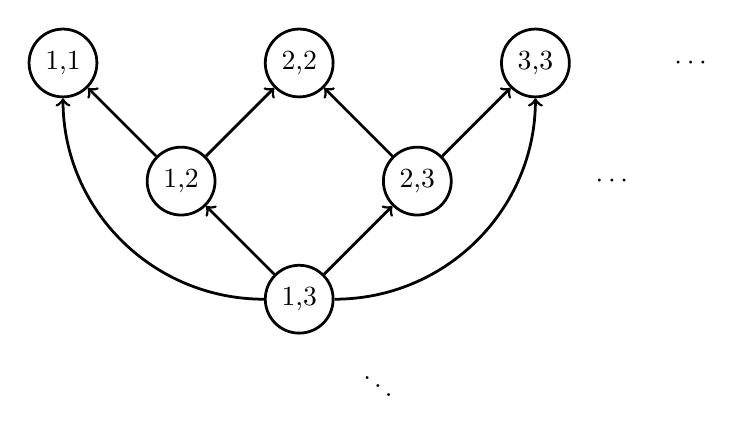
\begin{tikzpicture}[line width = 1pt,
                    solid/.style = {circle, draw, fill = black, minimum size = 0.3cm},
                    empty/.style = {circle, draw, fill = white, minimum size = 0.3cm}]
  \node [empty] (T11) at (4, 1) {1,3};
  \node [empty] (T21) at (2.5, 2.5) {1,2};
  \node [empty] (T22) at (5.5, 2.5) {2,3};
  \node [empty] (T31) at (1, 4) {1,1};
  \node [empty] (T32) at (4, 4) {2,2};
  \node [empty] (T33) at (7, 4) {3,3};

  \draw [->] (T11) -- (T21);
  \draw [->] (T11) -- (T22);
  \draw [->] (T21) -- (T31);
  \draw [->] (T21) -- (T32);
  \draw [->] (T22) -- (T32);
  \draw [->] (T22) -- (T33);
  \draw [->] (T11) edge [bend left=45] (T31);
  \draw [->] (T11) edge [bend right=45] (T33);

  \node at (5, 0) {$\ddots$};
  \node at (8, 2.5) {$\cdots$};
  \node at (9, 4) {$\cdots$};
  \end{tikzpicture} \par
  \end{centering}
  \normalsize
  \vspace{0.3cm}

  It has $\displaystyle \frac{n(n+1)}{2}$ vertices and $\displaystyle \sum_{i=0}^{n-1} 2n(i-n) = \frac{(n-1)n(n+1)}{3}$ edges. \par
  The edges are $\langle(i, j), (i, k)\rangle$ and $\langle(i, j), (k + 1, j)\rangle$, where $1 \leq i < j \leq n$ and $i \leq k < j$.

  \section{[TC] Problem 15.3-3}
  Yes. We have to choose a split with maximized number of scalar multiplications, each choice leaving two subproblems to be solved. Now we are going to prove that this is an optimal substructure.\par
  Suppose that one of the subproblem solutions used in the optimal solution is not optimal, i.e. there exists some solution to a subproblem which needs more scalar multiplications. Replacing the solution for the subproblem with the optimal one gives a solution with more scalar multiplications, which leads to contradiction. Therefore, this problem exhibit optimal substructure.

  \section{[TC] Problem 15.3-5}
  Here is a counterexample, where the final solution is optimal, but the solution to its subproblem is not optimal. \par
  Assume that the pieces of length 1, 2, 3, 4, 5 are worth 5, 1, 1, 1, 1, respectively, and each kind of piece should appear no more than twice. Consider cutting up a rod of length 5 to pieces to obtain the maximum revenue. We can easily verify that cutting the rod into pieces of length 1, 3, 1 obtains the maximum revenue. In this solution, the subproblem is to cut a rod of length-4, whose solution is 1, 3, which is not optimal (1, 1, 2 is an optimal solution). Therefore, the optimal-substructure property described in Section 15.1 no longer holds.

  \section{[TC] Problem 15.3-6}
  When $c_k = 0$, let $d_i$ denote the maximum amount of currency $i$ that we can achieve by a sequence of exchanges. $d_1$ is the amount of currency 1 you initially have. Then $d_j$ is the maximum of $d_i \times r_{ij}$ with respect to $i$, where $j$ is the index of the currency which can be exchanged for currency $j$. Suppose that the subproblem solution, say $d_{i_0}$, used in the optimal solution is not optimal, i.e. there exists $d_{i_1}$, such that $d_{i_1} > d_{i_0}$. Replacing $d_{i_0}$ for $d_{i_1}$ gives a better sequence of exchanges, which lead to contradiction. Therefore, the problem exhibits optimal structure when $c_k = 0$. \par
  When $c_k$ are arbitrary values, we can find a counterexample. Assume that you initially have $10.0$ units of currency 1, the exchange rates are $r_{1,2} = 2.0, r_{1,3} = 3.0, r_{1,4} = 0.0, r_{2,3} = 2.0, r_{2,4} = 0.0, r_{3,4} = 1.0$, and the commissions are $c_1 = 0.0, c_2 = 5.0, c_3 = 20.0$. We can verify that $\langle 1,3 \rangle, \langle 3,4 \rangle$ is a best sequence of exchanges. However, $\langle 1,3 \rangle$ is not the optimal solution to the subproblem exchanging currency 1 for currency 3. $\langle 1,2 \rangle , \langle 2,3 \rangle$ is a better solution. Therefore, when commissions are arbitrary, the problem does not necessarily exhibit optimal structure.

  \section{[TC] Problem 15.4-3}
  \begin{codebox}
  \Procname{$\proc{Memoized-LCS-Length}(X, Y)$}
  \li $m \gets \attrib{X}{length}$
  \li $n \gets \attrib{Y}{length}$
  \li \For $i \gets 0$ \To $m$
  \li \Do \For $j \gets 0 $ \To $n$
  \li     \Do $c[i, j] \gets \NULL$
  \li         $b[i, j] \gets \NULL$
          \End
      \End
  \li $\proc{Lookup-Length}(X, Y, m, n)$
  \li \Return $c$ and $b$
  \end{codebox}
  \begin{codebox}
  \Procname{$\proc{Lookup-Length}(X, Y, i, j)$}
  \li \If $c[i, j] \neq \NULL$
  \li \Do \Return $c[i, j]$
      \End
  \li \If $i \isequal 0$ or $j \isequal 0$
  \li \Do $c[i, j] \gets 0$
  \li \ElseIf $X[i] \isequal Y[i]$
  \li \Do $c[i, j] \gets \proc{Lookup-Length}(X, Y, i-1, j-1)+1$
  \li     $b[i, j] \gets $ ``$\nwarrow$''
  \li \ElseIf $c[i-1, j] \geq c[i, j-1]$
  \li \Do $c[i, j] \gets \proc{Lookup-Length}(X, Y, i-1, j)$
  \li     $b[i, j] \gets $ ``$\uparrow$''
  \li \Else
  \li     $c[i, j] \gets \proc{Lookup-Length}(X, Y, i, j-1)$
  \li     $b[i, j] \gets $ ``$\leftarrow$''
      \End
  \li \Return $c[i, j]$
  \end{codebox}

  \section{[TC] Problem 15.4-5}
  \begin{codebox}
  \Procname{$\proc{LIS}(X)$}
  \li $n \gets \attrib{X}{length}$
  \li let $b[1 \twodots n, 1 \twodots n]$ and $m[1 \twodots n, 1 \twodots n]$ be new tables \Comment $\displaystyle m[i, j] = \min_{\substack{1 \leq k_1 < \cdots < k_j \leq i \\ X[k_1] \leq \cdots \leq X[k_j]}} X[k_j]$
  \li $m[1, 1] \gets X[1]$
  \li \For $i \gets 2$ \To $n$
  \li \Do $m[i, 1] \gets \proc{min}(X[i], m[i-1, 1])$
      \End
  \li $i \gets 1$
  \li \While $m[i, n] \neq +\infty$
  \li \Do $i \gets i+1$
  \li     $m[i, 1] \gets +\infty$
  \li     \For $j \gets 2$ \To $n$
  \li     \Do \If $X[j] \geq m[i-1, j-1]$ and $X[j] < m[i, j-1]$
  \li         \Do $m[i, j] \gets X[j]$
  \li             $b[i, j] \gets$ ``$\nwarrow$''
  \li         \Else
  \li             $m[i, j] \gets m[i, j-1]$
  \li             $b[i, j] \gets$ ``$\uparrow$''
              \End
          \End
      \End
  \li \Return $b$ and $i - 1$ \Comment $i-1$ is the length of LIS
  \end{codebox}
  This procedure fills tables $m$ and $b$ whose sizes are at most $n \times n$, so the running time is $O(n^2)$.
  \begin{codebox}
  \Procname{$\proc{Print-LIS}(X, b, i, j)$}
  \li \If $i \isequal 1$
  \li \Do print $X[i]$
  \li     \Return
      \End
  \li \If $b[i, j] \isequal $ ``$\nwarrow$''
  \li \Do $\proc{Print-LIS}(X, b, i-1, j-1)$
  \li     print $X[i]$
  \li \Else
  \li     $\proc{Print-LIS}(X, b, i, j-1)$
      \End
  \end{codebox}
  The initial call is $\proc{Print-LIS}(X, b, l, \attrib{X}{length})$, where $l$ is the length of LIS.

  \section{[TC] Problem 15.5-1}
  \begin{codebox}
  \Procname{$\proc{Construct-Optimal-BST}(root)$}
  \li $n \gets $ length of the first dimension of $root$
  \li print ``$k$'' $_{root[1, n]}$ ``is the root''
  \li $\proc{Recursive-Construct-Optimal-BST}(root, 1, root[1, n] - 1, \const{Left})$
  \li $\proc{Recursive-Construct-Optimal-BST}(root, root[1, n] + 1, n, \const{Right})$
  \end{codebox}
  \begin{codebox}
  \Procname{$\proc{Recursive-Construct-Optimal-BST}(root, i, j, p)$}
  \li \If $i > j$
  \li \Do \If $p \isequal \const{Left}$
  \li     \Do print ``$d$'' $_j$ ``is the left child of $k$'' $_{j+1}$
  \li     \Else
  \li         print ``$d$'' $_j$ ``is the right child of $k$'' $_{i-1}$
          \End
  \li \Else
  \li     \If $p \isequal \const{Left}$
  \li     \Do print ``$k$'' $_{root[i, j]}$ ``is the left child of $k$'' $_{j+1}$
  \li     \Else
  \li         print ``$k$'' $_{root[i, j]}$ ``is the right child of $k$'' $_{i-1}$
          \End
  \li     $\proc{Recursive-Construct-Optimal-BST}(root, i, root[i, j] - 1, \const{Left})$
  \li     $\proc{Recursive-Construct-Optimal-BST}(root, root[i, j] + 1, j, \const{Right})$
      \End
  \end{codebox}

  \section{[TC] Problem 15-4}
  Assume that for all $1 \leq i \leq n$, $1 \leq l_n \leq M$. Let $m[i]$ denote the minimum sum over several lines containing the first $i$ words, including the last line. We have the following recursive formula:
  $$  m[i] = \min_{\substack{1 \leq j \leq i \\ l_{i-j+1} + \cdots + l_{i} + j - 1 \leq M}} m[i-j] + \left(M - j + 1 - \sum_{k = i-j+1}^{i} l_k  \right)^3 $$
  with initial condition $m[0] = 0$. \par
  Since the number of the extra space characters in the last line should not be added, the final answer is
  $$ \min_{l_{k} + \cdots + l_{n} + n - k \leq M} m[k - 1] $$ \par
  Then procedure $\proc{Printing-Neatly}(l, n, M)$ on the next page, returns a stack $T$, storing the indices of the words, after each of which there is a new line. The running time is $O(n^2)$, and the space requirement is $\Theta(n)$.
  \begin{codebox}
  \Procname{$\proc{Printing-Neatly}(l, n, M)$}
  \li let $m[0 \twodots n]$ be new array
  \li $m[0] \gets 0$
  \li \For $i \gets 1$ \To $n$
  \li \Do $S \gets M + 1$
  \li     $m[i] \gets +\infty$
  \li     \For $j \gets 1$ \To $i$
  \li     \Do $S \gets S - l_{i-j+1} - 1$
  \li         \If $S < 0$
  \li         \Do \kw{break}
              \End
  \li         \If $m[i-j] + S^3 < m[i]$
  \li         \Do $m[i] \gets m[i-j] + S^3$
  \li             $s[i] \gets i-j$
              \End
          \End
      \End
  \li $a \gets +\infty$
  \li $S \gets M + 1$
  \li \For $i \gets n-1$ \Downto $0$
  \li \Do $S \gets S - l_{i+1} - 1$
  \li     \If $S < 0$
  \li     \Do \kw{break}
          \End
  \li     \If $m[i] < a$
  \li     \Do $a \gets m[i]$
  \li         $j \gets i$
          \End
      \End
  \li let $T$ be a new empty stack
  \li \While $j \neq 0$
  \li \Do $\attrib{T}{push}(j)$
  \li     $j \gets s[j]$
      \End
  \li \Return $T$
  \end{codebox}
\end{document}
